\chapter{Problem Elaboration}

\section{Previous work}
This thesis and its motivation derived from previous work with hybrid games at NTNU, as mention in chapter \ref{ch:introduction}. In particular, Don\'t Panic was well received, but implementation was time consuming and setup during play proved difficult for players\cite{di2012don}. 

Other work done regarding hybrid games are often centered around tabletops\footnote{With \emph{tabletop} we refer to a table computer, such as Microsoft Surface 1.0 or Samsung SUR40} as the central component of the game. Weathergods\cite{bakker2007weathergods}, KnightMage\cite{magerkurth2004towards} and False Prophets\cite{mandryk2002false} are examples of these. Most of these report a positive feedback from users, inclining that hybrid games indeed can utilize the best from both regular and digital games. An article evaluating tabletop game experience for seniors even claim they enjoy hybrid games and get more immersed than with regular games \cite{al2008designing}.

Two framework has been previously developed for creating tabletop board games: ToyVision\cite{marco2012toyvision} and ReacTIVision\cite{kaltenbrunner2007reactivision}. However, their relevance might be dwindling, as tabletops for private use has near to disappeared. Most of the existing work regarding tabletop games was done in the period 2004-2010. Since then, there has been little development around tabletop games and tabletops in general, at least that target to the private consumer marked. Microsoft PixelSense\footnote{Microsoft PixelSense: Microsofts initative for tabletops.}, and their accompanied hardware, Samsung SUR40 is retired, according to their own websites\footnote{\href{http://www.samsung.com/uk/business/business-products/smart-signage/specialised-display/LH40SFWTGC/EN}{www.samsung.com/uk/business/business-products/smart-signage/specialised-display/LH40SFWTGC/EN} displays Samsung SUR40 as no longer available.}. We speculate that the high cost of aqcuiring tabletop devices\footnote{Samsung SUR40 currently goes for about 5000 USD on eBay market} has played a large role.

Hybrid games without tabletops has also been created. The game \emph{"In Search of the Amulet"}\cite{magerkurth2012hybrid} an 8x8 tiled board  implemented with rfid tags was used together with rfid readers inside digital player pawns. The pawns detected its movement and location on the board, and reported it to a computer. Each player here had each their computer functioning as a private space and allowing them to do actions without the other player knowing. In addition, a "public" screen showed information visible for both players. One of the challenges here was the potential intruising effects of the displays, and it was deliberately made to require as little as possible interaction with the digital components in order to uphold the social aspect. The article does not mention any hybrid game platforms being used.

\subsection{Summary}
Hybrid games of various kinds has been tested, prototyped and developed previously. From those articles we've seen, there has been nothing but  positive feedbacks from users, who have found such games entertaining and immersive.

Platforms for developing hybrid games more easily has been made, but these are centered around tabletop environments, which is not suitable for our task, due to their high aqusition cost.

With the exception of \emph{In Search of the Amulet}\cite{magerkurth2012hybrid}, we've been unable to find previous work of hybrid games with simple digital pawns independant of a tabletop device. We have been completely unable to find hybrid game platforms similar to the one we've planned to develop.

\section{Characteristics of board games} \label{sec:boardgames_commonalities}

In this section we will analyse three different board games to identify and classify typical components of the board games. The purpose of this is to identify classic types of interactions and components in board games, so that we can focus on the central elements to implement in our platform. 

At the end we summarize the elements we've identified. The characteristical concepts of board games are described in subsection \ref{subsubsec:boardgame_concepts}, while the physical components common for board games can be found in subsection \ref{subsubsec:boardgame_components}. 

The three board games we've chosen is Lords of Waterdeep, Monopoly and Don't Panic. These are chosen to cover common, but different types of board games. Lords of Waterdeep is a classic Dungeons and Dragons game, making use of typical "advanced" board game dynamics, while Monopoly is a simpler common type of board game, employing many standard actions and elements. Don't Panic has been chosen as an existing hybrid board game.

\subsection{Monopoly}
Monopoly is a widely popular property trading game. Players acquire properties and money through chance cards, landing on property tiles and completing "laps" on the board. They charge each other money for the "use" (landing on) their land. Players lose by going "bankrupt", which is when their assets amount to less than 0 amount of money. The \textbf{winner is declared when} all other players are bankrupt.

\begin{figure}[ht]
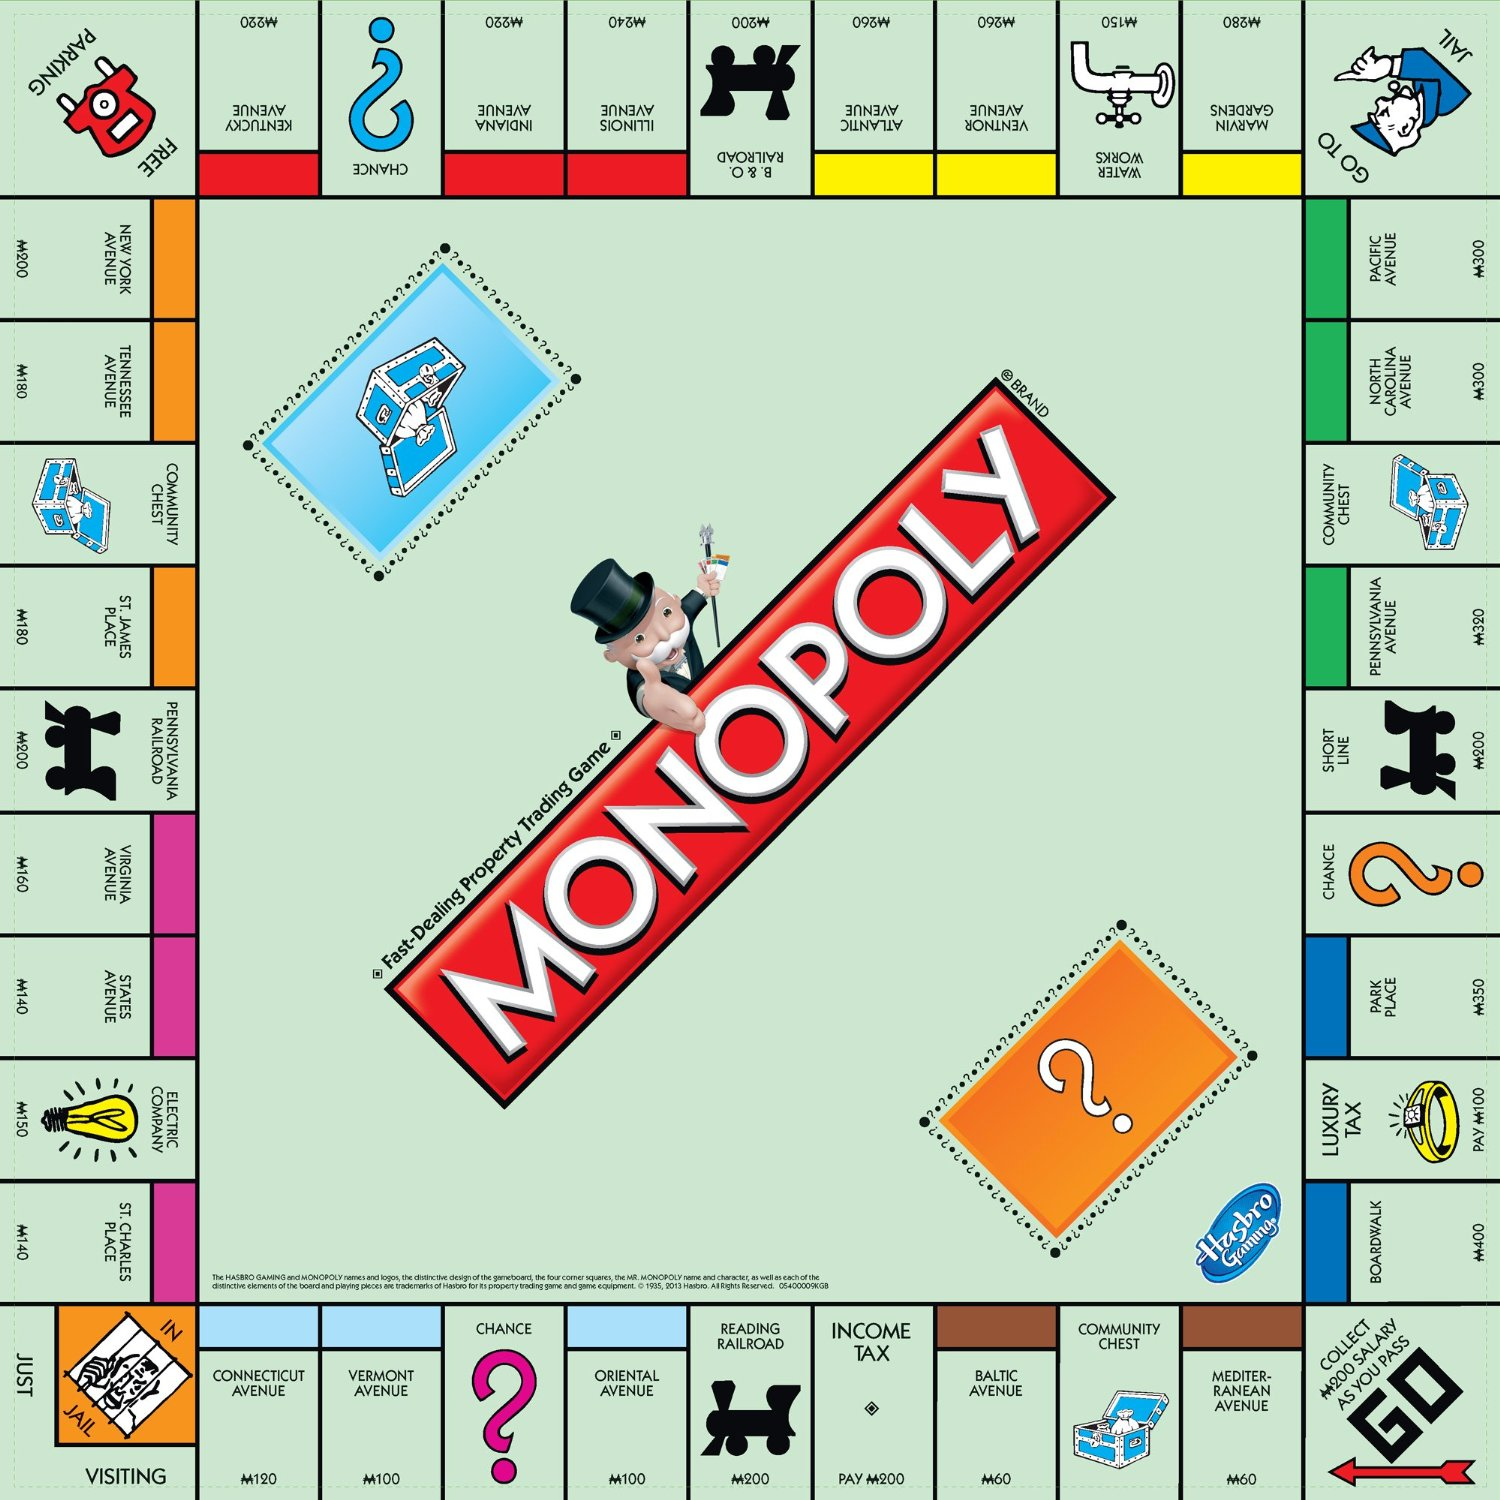
\includegraphics[width=12cm]{img/monopoly_board}
\centering
\caption{A version of Monopoly from Parker Brothers. Player pawns move from one to the next of the 40 tiles clockwise using two six sided dices.}
\label{fig:monopoly_board}
\end{figure}

The Monopoly \textbf{board} consists of roughly 40 discrete \textbf{tiles} as shown in figure \ref{fig:monopoly_board}. Each player has a \textbf{pawn} that represents them, which they move about the board with. The movement is determined by a roll of \textbf{dices}. Monopoly is \textbf{turn-based}, which means players take turn to throw the dices, moving their pawns, and completing a set of possible \textbf{actions} they can choose from, determined from the tile they land on. 

Each action usually involves buying, paying or exchanging  \textbf{resources} in form of money or stocks – which are placed in an inventory of each player. The inventory is a \textbf{private space} which contains the resources belonging to that player. Players starts the game with some initial resources in their inventory, but most are acquired during the game play. Resources are represented in form of two sorts of \textbf{informational tokens}: stocks and monopoly money. 

In short, the goal of the game is to maximize the acquisition of resources.

\subsection{Lords of Waterdeep} \label{subsec:LoW}
Lords of Waterdeep (LoW) is a \textbf{turn-based} game from the Dungeons and Dragons series, where players fight as a Lord in order to control a city. The goal of the game is to maximize the number of \textbf{points}. which are obtained mainly by completing quests. Quests are completed by obtaining a spesific combination of different adventureres in addition to a quest-card. 

In addition to quests and resources held by a player (marked red in figure \ref{fig:lords_board}), each player also is a spesific Lord (\textbf{Role}) which gives bonus points to certain quests for that player. LoW also include a type of cards called Intrigue, which can be used in various advantageous ways.

\begin{figure}[ht]
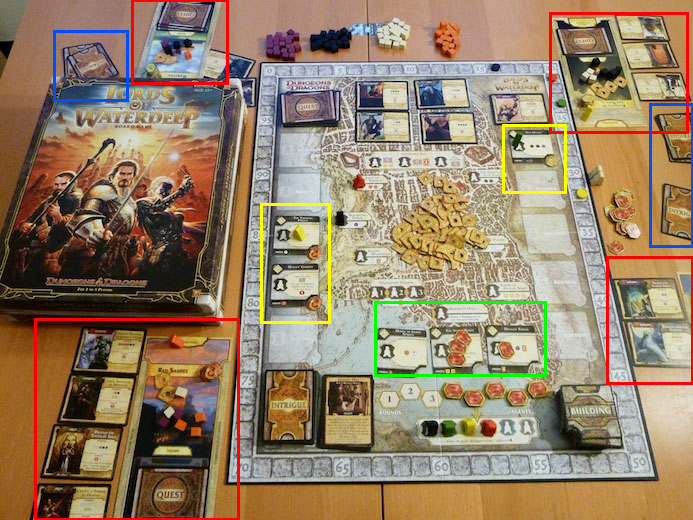
\includegraphics[width=12cm]{img/lords_board_marked}
\centering
\caption{Lords of Waterdeep. Players have multiple pawns and place them on available tiles as they please. New tiles (yellow) can be bought into the game allowing for a greater set of possible actions. Each player has both a visible (red) and hidden (blue) private space.}
\label{fig:lords_board}
\end{figure}

The Lord and Intrigue-cards are held in a \textbf{hidden private space}, a space that is not visible to other players other than the holder. Compared to games that doesn't have such dynamic, this hidden space introduces a new dimension to the game, as players hold different information.

LoW also make use of \textbf{rounds}. After all players have placed their pawns on the board, and actions has been completed, a round is over. All pawns are being put back into the inventory of each player, and points given by acquiring new tiles (buildings) are increased. After the fourth round, players are given an extra pawn, and the game ends after the eight round.

Another interesting component of LoW is its \textbf{dynamic board}. Of of the initial tiles can be used by players that wish to buy a new tile. The new tile will be an available in that and all the remaining rounds, and will reward the buyer upon usage.

\subsection{Don't Panic}
Don't Panic (DP) is a \textbf{cooperative} board game with different zones, where panic can emerge among "people" and spread to nearby zones. The players, unlike in Monopoly or LoW, work together in an effort to reduce panic. In DP, the players attempt to calm a situation down, and loses if the panic level goes beyond a certain threshold.

\begin{figure}[ht]
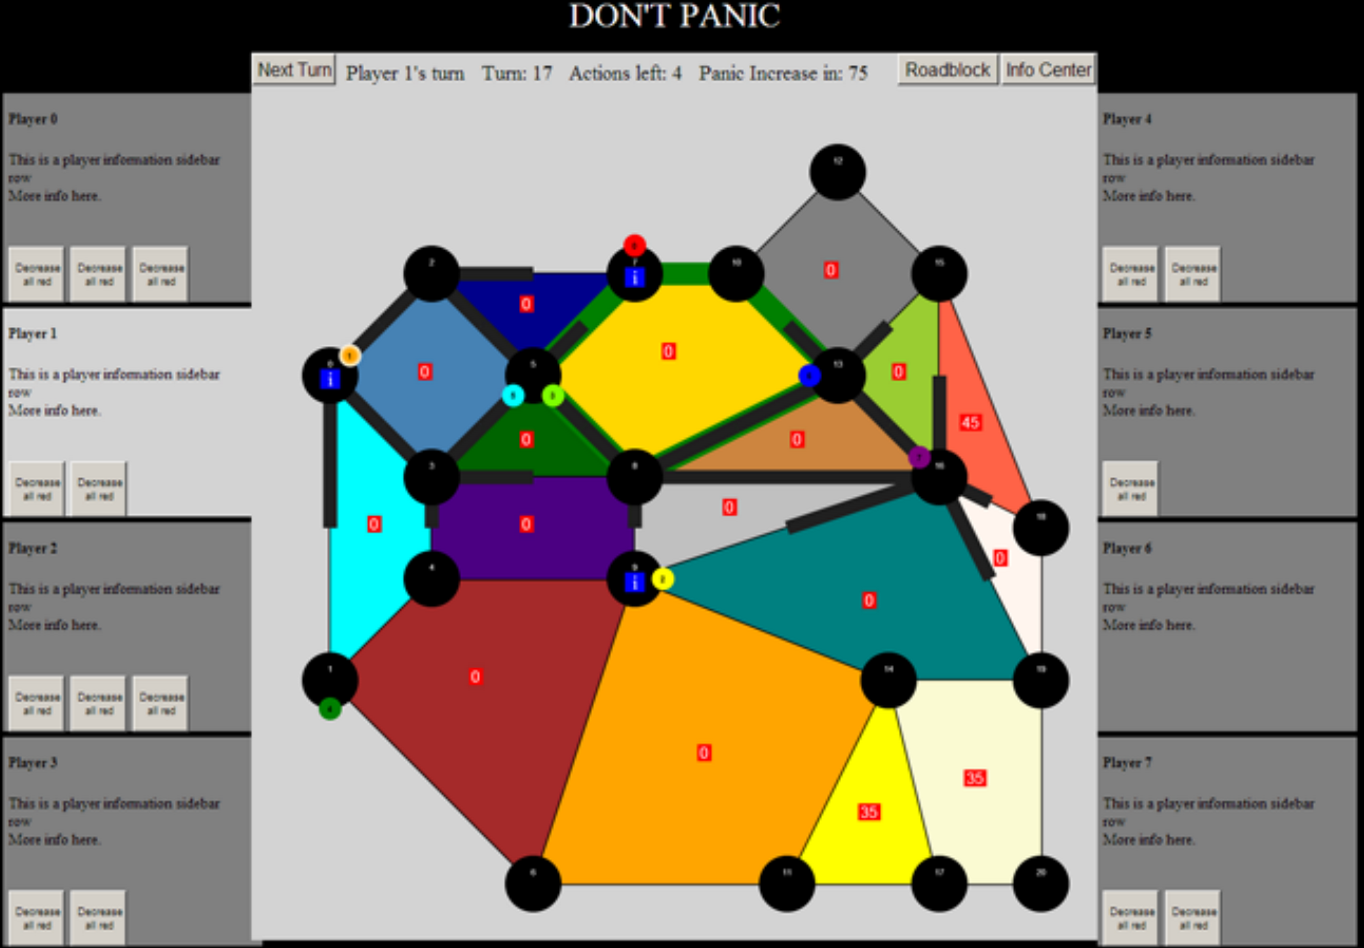
\includegraphics[width=12cm]{img/dont_panic_interface}
\centering
\caption{Digital version of Don't Panic. The map is divided into zones with a respective panic level. Player pawns locate themselves on the different nodes, and attempt to lower and contain the panic.}
\label{fig:dont_panic_board}
\end{figure}

Each player is presented by a pawn (colored circles in figure \ref{fig:dont_panic_board}) located on tiles (black nodes), and takes turn to draw 2 informational cards, 2 event cards and complete 4 "actions". Event cards are challenges which the players have to deal with on their turn, and can be resolved by "actions" or the use of informational cards. The informational cards are a form of resource that can (optionally) be used on a players turn. 

The 4 "actions" performed by players on each turn can be chosen from a set of actions containing movement of pawn, movement of people between zones, set up or remove road blocks to contain panic, as well as building an information center. Each player is also randomly given a role at the start of the game, which gives them an advantage on a spesific type of action. 

Once the game starts, a \textbf{timer} is initialized, counting down from a certain amount of minutes. Once the timer rings, panic levels are increased, and can spread between zones. This introduces a dimension of stress or hurry to the game, as playing faster gives an advantage.

\subsection{Summary: concepts} \label{subsubsec:boardgame_concepts}
\textbf{Players and Teams}: Board games are typically played in social settings with two or more players. In many board games such as Monopoly, each player is represented with a physical object called "pawn". In LoW, we saw that this is not the case, but rather had several agents that acted on behalf of the player.

Commonly, every player play each against other and is as such on team with only themselves, such as in Monopoly or Low. In other games, such as DP, several or all players can also play on teams with each other, fight common enemies even including the game itself.

\textbf{Roles and skills} are player-spesific properties that deviate from the standard rules of the game, and can give advantages or disadvantages in different aspects of the game. In DP, each player is assigned a Role by random, which gives them advantages in performing certain actions. For example, a driver can move more people out of paniced areas. Similarily in LoW, each player is assigned a Lord card (character) by random, which increases the points granted upon completing certain quests. LoW also has special quests that provide an advantage for the rest of the game (skill). For example, completing the quest "Quell Merchenary Uprising" will provide the player with two extra points for every other quest of the same type he or she completes.

\textbf{Public and private spaces}: Public and private spaces are the conceptual areas containing parts of the game that is interacted with by all or one of the players. Public spaces can be interacted with by all players, while each player has a private space that only that player can interact with. In Monopoly, question cards, dices and cards are a part of the public space, while money belong to the private spaces of each player.

\textbf{Hidden private space}, is the a private space that is not visible for other players. For example a hidden hand contains cards that are visible only to the holder of the cards. For example in LoW your Intrigue cards (uncommon advantageous actions you can perform) is hidden from other players. 

\textbf{Themes} provide a background story and explain the motivation and goal for the players. Both Monopoly, LoW and DP have themes that help relate the game to real world concepts and provide some story that can help players immerse them selves in the games. This is unlike games as Poker or Tic Tac Toe.

\textbf{Events} are special parts of the game that often go outside the normal flow of the game. In Monopoly, one of the tiles will send you to "jail". This includes a movement of the pawn that is not based on dices like the rest of the game, and gives an exception to the dice rolling and movement in the next turns. An event is also triggered when drawing question cards: winning the lottery or having to repair your houses go outside the normal flow of the game. In LoW, playing Intrigue cards will trigger events, allowing for players to take resources from others or imposing a mandatory quest upon other players. And in DP, Event Cards and playing Informational Cards can be categorized as events. Events are typically unpredictable, either by being in a shuffled deck of cards or played from a hidden private space.

\textbf{Resources} are assets belonging to a player. In Monopoly, the resources are Stocks, Money and Houses. Player controlled events, such as the Get Out of Jail Free Card (Monopoly) or Intrigue card (LoW) can also be considered resources. Resources are often made physical through Indicator Tokens (see \ref{subsubsec:boardgame_components}).

\textbf{Turns and actions}: In turn-based games each player takes turn to complete some actions, before the next person plays his turn. Each turn usually involves a scripted set of actions. In Monopoly, you must always roll two dices and move your pawn that amount of tiles. This is a mandatory action. The tile determines the next set of actions you can perform. Either 1) pay the owner rent (mandatory), if the tile is currently owned by anther player, 2) buy the stock (optional) if the tile is for sale, 3) draw a card and complete it's action (mandatory) if landing on a question-tile. In other words, turns are sets of actions, where each action can either be mandatory or optional, that can have a precondition, i.e. do this if that, and can be ordered, i.e. done in a speific order.

\textbf{Rounds} is a concept that some event or set of events will incur, usually that sets back the game in some way, after some critiera is met. In LoW, actions is performed via agents, which is "spent" once put on the board. When all agent actions are exhausted, the round is over, and agents are put back into their respective players private space so that they can perform actions on behalf of the player again. In DP, one can interpret the time between each alarm as a round. Once the round is over, panic is increased and potentially spread.

\textbf{Rules} tell us the possible interactions between game components: Which actions is involved in a turn? When is a round over? How can your pawn move around the board? When is a winner declared, or a player out of the game? Rules explicitly define the starting conditions upon starting the game, and are a central part of all games, as they dictate the flow of the game and define the bounderies of them.

\subsection{Summary: Physical components} \label{subsubsec:boardgame_components}

\begin{figure}[ht]
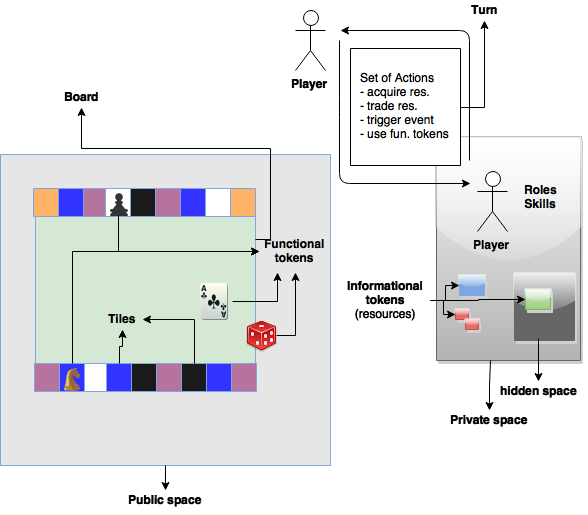
\includegraphics[width=12cm]{img/board_games_components}
\centering
\caption{Common components of board games. Board with tiles and functional tokens as a part of the public space, while informational tokens (resources) as part of each players private space, potentially hidden from view from other players. The game is progressed by players taking turn to acquire and trade resources, triggering events and interacting with functional tokens.}
\label{fig:board_games_components}
\end{figure}


\textbf{Board} is the surface used to play a board game. Most games have a unchanging board (Monopoly), while some have a modular board with varying layout in each session or while the game is played (LoW). The board consists of tiles and placeholders for other assets.

\textbf{Tiles} are discrete locations on the board. Which tile a player is located on, usually determines which set of \emph{actions} the player can perform. In Monopoly for example, a stock can only be bought when the the pawn is located on that spesific tile. In Don't Panic, it didn't determine which actions one could perform, but rather which part of the city the player could perform his actions upon. In some games, such as Monopoly and DP, movement is only allowed over adjecent tiles.

\textbf{Indicator tokens}, e.g. Gold, Wood, Stone, Gas, Money, Points, Stocks and Houses help keeping track of an informational aspect in the game. In Monopoly, the paper money is simply an indicator of how much resources owns, and stocks an indicator of the lots owner. It serves its purpose by holding some information, and as such simplifying the amount of information players have to remember and keep track of themselves.

These are simple tokens, as they are only representatational of some game information, and does not change the game state or provide interactive functionality like randomness. Such tokens can easily be replaced by a number value or position on a screen, as they are not interacted with other than changing owner.

\textbf{Functional tokens}, e.g. dice, cards and pawns play an active part in how the game unfolds. For example, a dice in provides randomness as a functionality to the player, while the timer in DP provide an aspect of time or hurry. Cards are the most common functional tokens, which can provide many types of events and exceptions to the standard flow of the game, as well as provide randomness through being shuffled and used in a drawable deck.

These tokens change the state of the game by opening or closing certain actions and aspects for players. Each of these tokens have a specialized functionality, and can not be implemented as generally as indicator tokens.

\newpage


\section{Life cycle and roles}
In this section we go through the life cycle of a game, from idea through creation to a playable augmented board game. We focus on the roles and their contributions and actions in creating and using the game, as was the case with the previous augmented board game created at NTNU, Don't Panic . In the next section we will look at the challenges linked with these activities. 

We have identified three roles: a \textbf{Game Designer}, who formalizes and defines the game. The end result from a game designers production is a playable paper prototype. A \textbf{Developer} takes this prototype and identifies and acquires suitable hardware pieces, designs the user interface to be used in the game controller and implements the game through the controller and the hardware tokens. A \textbf{Player} should then able to acquire, set up and play the game. These roles and their typical activities are illustrated in figure \ref{fig:LifeCycleGameDesigner}, \ref{fig:LifeCycleDeveloper} and \ref{fig:LifeCyclePlayer}. The activites that we will focus on in this thesis is marked in green.



\begin{figure}[ht]
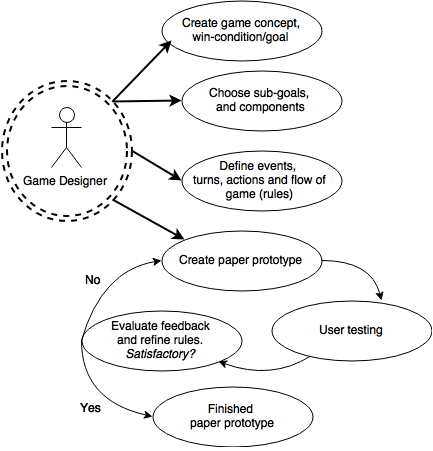
\includegraphics[width=8cm]{img/LifeCycleGameDesigner}
\centering
\caption{An overview over the responsibilities of the Game Designer in implementing hybrid board games. }
\label{fig:LifeCycleGameDesigner}
\end{figure}

\begin{figure}[ht]
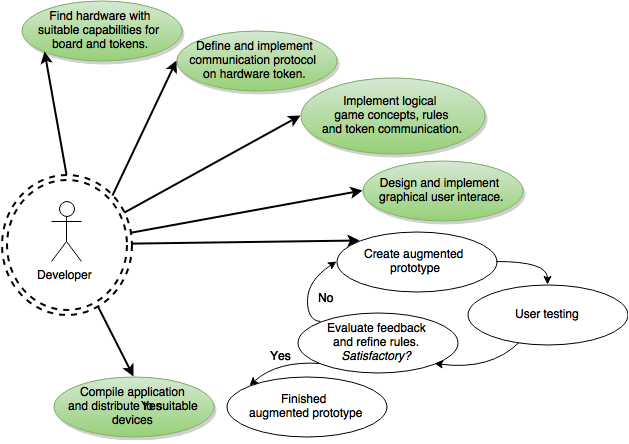
\includegraphics[width=12cm]{img/LifeCycleDeveloper}
\centering
\caption{An overview over the responsibilities of the Developer in implementing hybrid board games, after a finished paper prototype is provided by the game designer. The responsibilites marked with green are areas where we think AnyBoard can assist.}
\label{fig:LifeCycleDeveloper}
\end{figure}

\begin{figure}[ht]
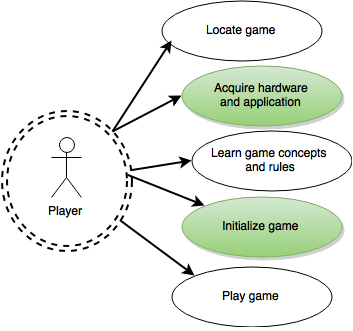
\includegraphics[width=7cm]{img/LifeCyclePlayer}
\centering
\caption{Main interactions from the view of a player in using hybrid board games. From previous experience in the testing of Don't Panic, replacing hardware tokens and game initialization (marked green) was too hard for non-technical players to receive a copy of the game.}
\label{fig:LifeCyclePlayer}
\end{figure}

\subsection{Designing}
The Game Designer starts with an idea, and details it through defining concepts, providing a motivation/goal, and giving the game clear rules and boundaries. The end result from the game designer should be a playable paper prototype of the board game. The following questions are the main questions that a game designer should be able to provide answers for (short Monopoly example answer in emphazised text):
\begin{enumerate} \label{design_cycle}
\item How are the teams - who is playing against who? \emph{Every player for themselves}
\item What is the game concept? Why are the players playing for/the goal? \emph{Achieving monopoly by making your opponents bankrupt}
\item What resources and game objects does the game consist of? Which is manifested in physical tokens? \emph{Stock, Money, Pawns, Houses, Hotel, Board, Question Cards}
\item What are the definite win- and lose conditions? \emph{You lose when you have no valuables left. Winner is the last player standing}
\item Through which actions does the game progress? \emph{Roll dice to change tiles. Tiles can be bought, traded, trigger event, paid rent for staying at. Each player takes it turn to complete a set of actions}
\item What are the initial set-up conditions of the game? \emph{Every player start at go tile with the same initial amount of resources.}
\end{enumerate}
These answers is described in detail and usually goes through several iterations (often with user feedback), before he or she comes to a final version that should be able to be played on a paper prototype. This iteration and refinement process could also be skipped, and rather done in the next phase, after implementating the game as an augmented board game.

\subsection{Implementing}
The Developer should have a clear description of the board game from the Game Designer. He will convert the game into an augmented version, by indentifying suitable digital tokens and interfaces, and implement the game logic into the necessary tokens and devices. A user friendly interface is necessary to allow players to initiate and play the game, and the applications should be distributed in a way that makes it easy to acquire. In short, the Developer takes the game from a finished concept to a finished product. This is shown in figure  \ref{fig:LifeCycleDeveloper}.

We have here assumed a case where a game controller (Phone, Tablet, Computer) and a set of tangible, digital hardware tokens has been used to create an augmented version of the board game. The Developers main responsibilites, are (examples are shown in emphasized text):
\begin{enumerate} \label{develop_cycle}
\item Translate the required token expressions and interactions into a clear grammar. \emph{Pawn can be placed on board and should notify of location. Pawn can show color and vibrate.}
\item Find or make digital hardware tokens that are capable of necessary token expressions. \emph{"rfduino" device should be capable of our requirements.}
\item Define and implement a communication protocol between tokens. \emph{Make "rfduino" accept "SET COLOR RED" over serial bluetooth and execute the corresponding expression.}
\item Implement game concepts, rules and token communication. \emph{Creating the logical representations of "Stock", "Money", "Board" etc, a token communicator object, and procedures to initiate the game and handle "paying rent".}
\item Designing and implementing the GUI. \emph{Creating a menu with buttons to run initiate procedure, read rules, and exit game. Designing an choice screen to handle trades between players}
\item Compile the game so it is distributable. \emph{Compile to iOS and Android files and distribute on App Store and Google Play}
\end{enumerate}
Prior to the compiling and distribution the game, the Developer should go through an iteration and refinement process to ensure the quality of the game. The game should now be ready for players to acquire and play the game.

\subsection{Playing}
A Player of the game is not involved in the creation of the game, but is a consumer of the finished product, a player of the augmented boardgame. In acquiring and playing the game, he or she will typically go through the following steps (examples in emphazised text, illustrated in figure \ref{fig:LifeCyclePlayer}):
\begin{enumerate} \label{play_cycle}
\item Locate the game. \emph{Hear of game from a friend, and go to its website.}
\item Acquire hardware and application. \emph{Order the necessary tokens online, and download a corresponding application from App Store}
\item Learn game rules. \emph{Read the game manual, and a FAQ on the applications website}
\item Initiate Game. \emph{Turn on tokens, open phone application, establish communication between tokens, and set up initial game conditions}
\item Play game. \emph{Interact with tokens (and phone application) according to the game rules}
\end{enumerate}





\section{Challenges} \label{sec:problem_challenges}

In this section, we will look at some of the challenges that each role face today when creating hybrid games, such as Don't Panic. These will strongly influence us when making high level requirements in the next section.

\subsection{Game Designer}
The work of the Game Designer is creating an entertaining experience. It's a creative process, with few rules that dictates how things ought to be. The challenges for a game designer is finding the inspiration and ideas necessary to create a good game concept. Even with a good concept, the designer should find volunteers to play the game and give adjustive feedback. Once a prototype is polished enough for the designer to be satisfied, the rules and concepts must be defined in such a way that the developer is able to translate it to a program.

\begin{itemize}
\item Finding inspiration for the game concept and ideas can be hard.
\item The game designer must find volunteers that can provide user feedback to help refine the game.
\item The game designer should preferably have knowledge of typical game concepts.
\item Defining the game clearly enough to be computer translated.
\end{itemize}

\subsection{Developer}
There exists few suitable digital tokens for hybrid board games. As with the augmented version of Don't Panic, this can lead to a large amount of time being spent finding or making custom tokens (number 2), and establishing communication (number 3 and 4) between the tokens. This also requires knowledge of low level programming. 

There are few existing game tools aimed for board games. Among them, there are no tools geared for using tangible tokens. A developer might therefore have to build the board game concepts from scratch (4, 5), and modify the tools to support the tangible aspect (4).

\begin{itemize}
\item Developers must know both high level and low level code
\item Large amount of time is used creating custom hardware tokens
\item Communication between tokens must be built from scratch.
\item Existing game tools is likely to require modification to support the tangible aspect of hybrid board games.
\item End-users (Players) use various devices, operating systems and screen sizes. It can be time consuming to support the different devices.
\item Licenses for game development tools can be costly.
\end{itemize}

\subsection{Player}
Challenges of the Player: First, the lack of mature components make it hard to initiate the game (number 4 in). In Don't Panic, set up of the game required technical knowledge and was time consuming. It required starting an off-site server, and starting scripts manually on some of the game tokens. Second, the equipment used was custom made, and could as such not be easily replaced (number 2).  Since the equpment was custom made, it could not be reused for other purposes without reprogramming. If a Player wish to acquire a second similar game, he must anticipate to buy another set of hardware (number 2). Having located and enjoyed one augmented board game, the lack of a an community or platform around hybrid board games can make it difficult to locate new such games (number 1)

\begin{itemize}
\item In existing prototypes it has been hard for players to initiate a game, as the setup have required techical knowledge.
\item Hardware purchased for one game has not been suitable for reuse in other games without reprogramming, which is both time consuming and requires technical knowledge.
\item Lack of community around hybrid board games, makes it hard to acquire and locate such games.
\end{itemize}

\section{Components and high level requirements}
\label{sec:high_level_requirements}

From the challenges in creating hybrid board games, we believe that an platform for creating augmented boardgames can all involved roles greatly. The role of a game designer requires knowledge of game concepts, and has a great challenge of creating an entertaining game and balancing randomness with skill and knowledge. A game designer could be assisted by helping the creative process or simplify the concepts that a board game can consist of. A game designer has technical challenges, and the lack of existing, suitable hardware tokens and tools for integrating them with a user friendly mobile surface can make the implementation of the game very time consuming. From testing Don't Panic, we know that acquisition of hardware tokens should be cheap, and games easier to set up. Tokens should also preferably be reusable to other games for people without technical knowledge. We also think that the marked for such games is too small to be easily discoverable.

\subsection{High level requirements}

We have chosen to focus mainly on the challenges of the developer, and assist him or her in the implementation process of hybrid board games.

\begin{itemize}
\item D1 - A \textbf{game developer} should be able to extend or remove parts of the AnyBoard platform, in order to suit his or her needs that are not originally covered by the platform.
\item D2 - A game developer should not be required to pay for creating games through the AnyBoard platform, in order to lower the barrier for using AnyBoard.
\item D3 - A game developer should not be required to rewrite his or her game in order to be supported on different platforms or screen sizes, so to minimize the development effort necessary to reach a broad audience.
\item D4 - A game developer should be assisted with guidance on how to compile and deploy the applications to Google Play (Android) and App Store (iOS), in order to simplify the development and distribution of games made with AnyBoard.
\item D5 - A game developer should be provided with an API for communicating with supported digital tokens, and not be required knowledge of low-level code, in order to lower the barrier for using the AnyBoard platform.
\item D6 - A game developer should be able to extend digital token support to new tokens with new features with example code and written guides, in order not to restrict the developer to a fixed set of tangible tokens.
\item D7 - A game developer should be provided with classes and abstractions for typical board game entities, such as boards, pawns, dices, cards and decks, in order to lower the development time.
\item D8 - A game developer should be provided with a basic set of visual elements for screen display, such as menus, cards, boards, pawns, timers and buttons, in order to lower the development time.
\item D9 - A game developer should be provided with signals and event handlers to simplify implementing responses to a players actions, and game events.
\end{itemize}
\begin{itemize}
\item P1 - \textbf{A player} should not be required to have technical competence in order to initialize a game made with AnyBoard, in order to lower the barrier for players to acquire an augmented board game.
\item P2 - A player should be able to reuse board game hardware to play other games with ease, in order to lower the barrier for players to try other hybrid board games once having acquired one.
\end{itemize}

\subsection{Main components}
We present here a broad idea for how we can fulfill these requirements and create tools to accomodate and help developers and players to create and use hybrid board games. A sketch of this can be seen in figure \ref{fig:high_level_components}.

\begin{figure}[ht]
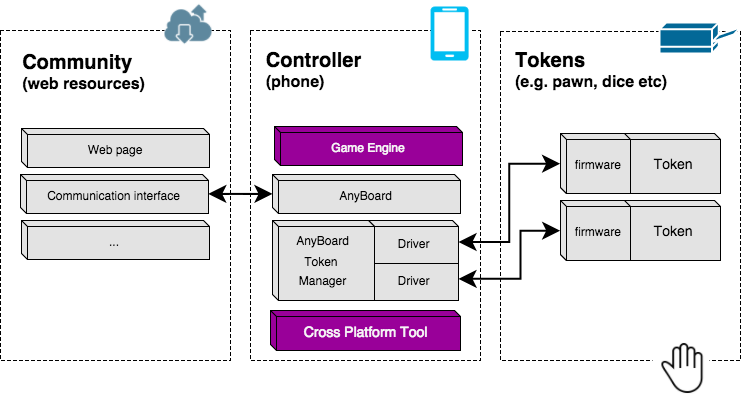
\includegraphics[width=12cm]{img/broad_architecture_idea.png}
\centering
\caption{High level components of AnyBoard.}
\label{fig:high_level_components}
\end{figure}

Game development tools and communities already exists, and hence the main part that makes the AnyBoard platform unique, is helping integrate the tangible tokens as a part of games. This is therefore the area of greatest importance. 

\emph{Standard example tokens}, with low level code implementing typical token capabilities, will be provided for developers that wish to create games with general token requirements. This token will communicate with a \emph{Token manager} on the application side that handles the communication between the game logic and physical devices. This component will provide a token API on the software side, so developers can listen to token-events and send commands without the knowledge of the low level code, as well as assist developers to create easy-to-use interfaces for connecting and initiating the game and game tokens.  \emph{(P1, D5)}

The Token manager is separated from any spesific token, and communicates through a \emph{device spesific driver}. A generic extendable driver will be provided to assist developers that wish to create their own tokens with other capabilities. \emph{(D1, D6)}

A \emph{Game engine} will provide tools that help the developer quickly create the components of his or her game. We wish to provide base components spesificly suited for hybrid board games, such as Board, Tile, Pawn, Dice etc, both the logical and visual \emph{UI} part. \emph{(D7, D8, D9)}

The AnyBoard software platform should be based on a \emph{cross platform tool} that enable games made with the AnyBoard to compile to different operating systems. \emph{(D3, D4)}

Several of these components exists already, and we aim to use open source, free-to-use, modular and well documented tools, so that a developer can pick apart the AnyBoard system and add capabilities where need be. \emph{(D1, D2)}

Lastly, a web-based home for AnyBoard can grow a community and provide information for all roles involved with hybrid board games. The AnyBoard platform could be downloaded from here, and tokens sold from a web store. It can also provide a knowledge base and tools for developers to assist each other. Through a \emph{Game Store} or an overview of hybrid board games, we hope to assist users with finding other games they can play, and an assistive IDE for game developers could help lower the knowledge barrier for new developers even further. \emph{(P2)}\footnote{A game store, or a web based IDE is a later stage than the AnyBoard platform presented in this thesis.}. 





\newpage